\documentclass[11pt]{article}

\usepackage{graphicx}

% Enable references to labels in the notes
\usepackage{xr-hyper}
\externaldocument{p328_notes}
\usepackage{hyperref}

% Sans fonts
\usepackage{sfmath}
\renewcommand{\familydefault}{\sfdefault}

\newcommand{\COURSE}{PHYS328W}
\newcommand{\LABNUM}{8}
\newcommand{\TITLE}{Common Emitter Amplifier}
\markright{\COURSE~Lab \LABNUM\ : \TITLE}

\setlength{\textwidth} {6.5 true in}
\setlength{\textheight}{9 true in}
\setlength{\hoffset}   {-0.75 true in}
\setlength{\voffset}   {-0.75 true in}
\setlength{\parindent} {12 pt}
\pagestyle{myheadings}

\begin{document}

\thispagestyle{empty}

\section*{\COURSE\ Lab \LABNUM\ : \TITLE}

This assignment relies on Section~\ref{sec:commonemitter} of the notes.

\begin{figure}[ht]
  \begin{center}
    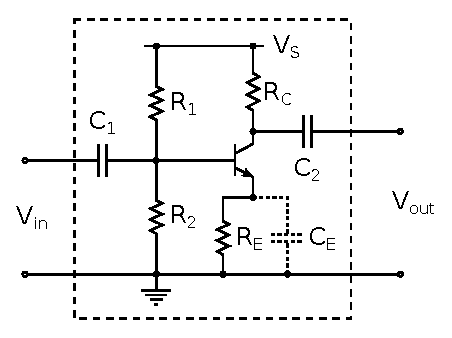
\includegraphics{commonemitter.eps}
    \caption{Schematic of an AC coupled common emitter amplifier.}
    \label{fig:commonemittercircuit}
  \end{center}
\end{figure}

\subsection*{Design}

Select resistor and capacitor values for the AC coupled common emitter
amplifier shown in Figure~\ref{fig:commonemittercircuit}, following the
process described in Section~\ref{sec:commonemitter} of the notes.
Design your amplifier to meet the following specifications, within
about 10\%, using available resistors and capacitors.
\begin{center}
\begin{tabular}{rc}
 Quiescent current & $I_C = 1$~mA \\
      Voltage gain & $A_v = -20$ \\
      Output range & $-5~\mathrm{V} \leq V_{out} \leq 5~\mathrm{V}$ \\
Signal frequencies & $f > 100$~Hz \\
\end{tabular}
\end{center}
Do all of your design calculations in your log book.

\subsection*{Experiment}

\begin{enumerate}
\item Collect the resistors and capacitors you need, and measure their
  values with a DMM.
  
\item Build the circuit you designed. If possible, use the transistor
  you studied in Lab~7.

\item Measure the quiescent collector current $I_C$, collector
  voltage $V_C$, base voltage $V_B$, and emitter voltage $V_E$, and
  compare them to what you expect based on your design calculations.
  
\item Use the function generator to supply a sinusoidal input signal
  $V_{in}$. Set the amplitude of the input signal to give a 1~V
  amplitude $V_{out}$.

\item Measure the voltage gain $A_v$ at several frequencies from 10~Hz
  to 1~MHz, concentrating your points in the low-frequency range where
  $A_v$ changes.

\item Determine the 3~dB point of the amplifier.
\end{enumerate}

\subsection*{Products}

Upload to Canvas a brief \LaTeX\ report in which you ...
\begin{itemize}
\item Include as a figure your $A_v$ vs. frequency plot.

\item Comment on the agreement between your design and measured values
  of the quiescent $I_C$, $V_C$, $V_B$, $V_E$, and the 3~dB point
  of the amplifier.

\item Include as a figure an image of the design calculations from
  your log book.
\end{itemize}

\end{document}
